\documentclass{standalone}
\usepackage{tikz}
\usetikzlibrary{patterns}
\usetikzlibrary{positioning}
\usetikzlibrary{patterns, positioning}
\usetikzlibrary{shapes.misc}
\usepackage[outline]{contour}
\contourlength{1.5pt} 
\usepackage[sfdefault]{ClearSans}

\begin{document}
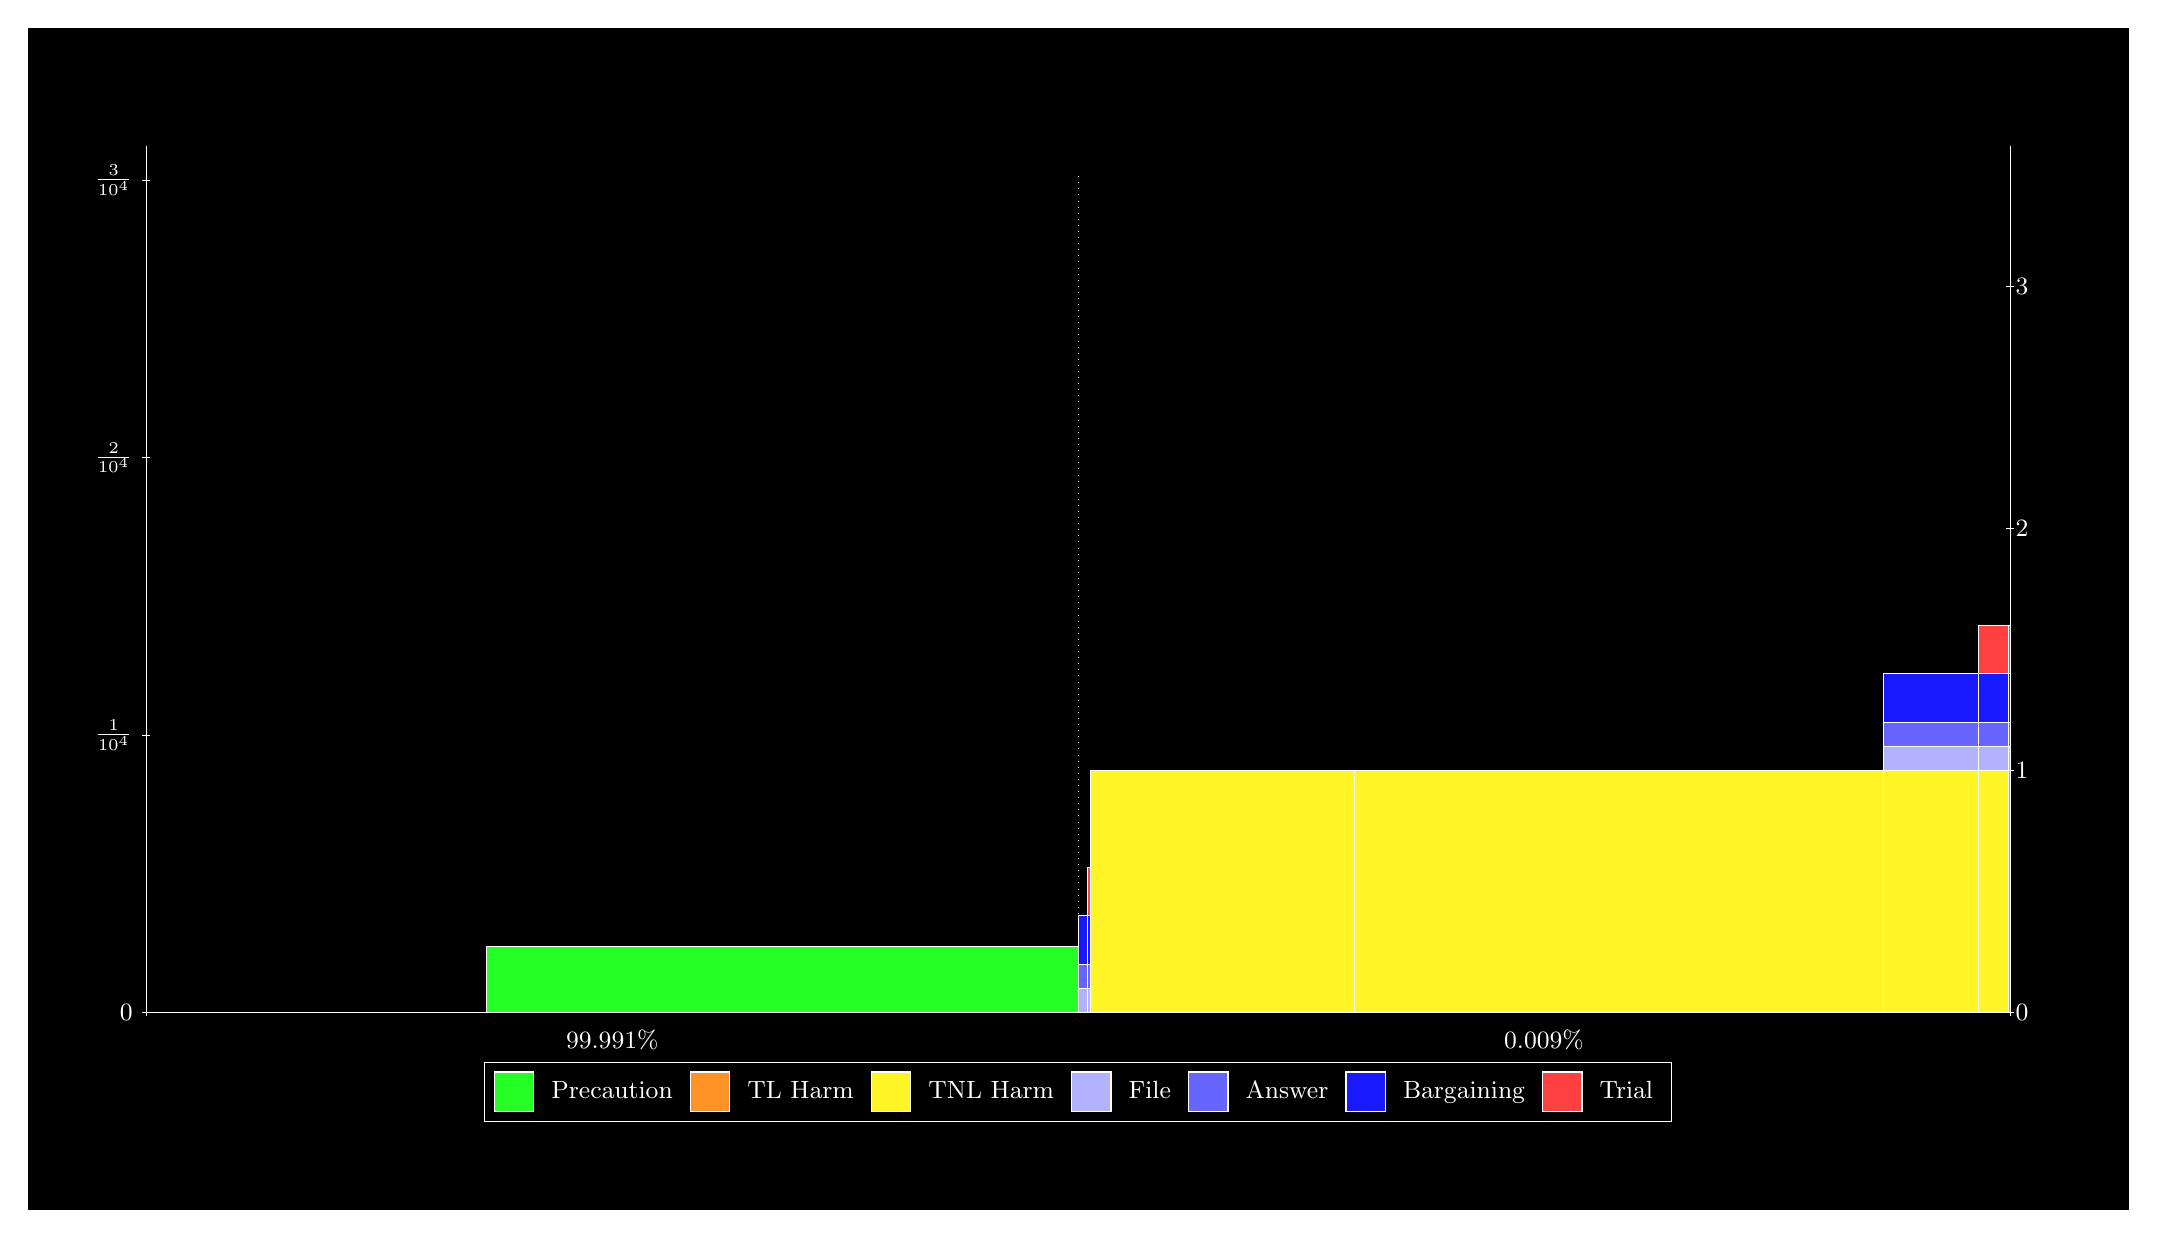
\begin{tikzpicture}
\draw[fill=black] (0,0) rectangle (26.667,15);
\draw[fill=green!85,draw=white,very thin] (5.8206,2.5) rectangle (13.333,3.3458);
\draw[fill=blue!30,draw=white,very thin] (13.333,2.5) rectangle (13.454,2.8074);
\draw[fill=blue!60,draw=white,very thin] (13.333,2.8074) rectangle (13.454,3.1148);
\draw[fill=blue!90,draw=white,very thin] (13.333,3.1148) rectangle (13.454,3.7295);
\draw[fill=blue!30,draw=white,very thin] (13.454,2.5) rectangle (13.494,2.8074);
\draw[fill=blue!60,draw=white,very thin] (13.454,2.8074) rectangle (13.494,3.1148);
\draw[fill=blue!90,draw=white,very thin] (13.454,3.1148) rectangle (13.494,3.7295);
\draw[fill=red!75,draw=white,very thin] (13.454,3.7295) rectangle (13.494,4.3443);
\draw[fill=yellow!85,draw=white,very thin] (13.494,2.5) rectangle (16.838,5.5738);
\draw[fill=green!85,draw=white,very thin] (16.838,2.5) rectangle (23.557,2.5001);
\draw[fill=yellow!85,draw=white,very thin] (16.838,2.5001) rectangle (23.557,5.5739);
\draw[fill=yellow!85,draw=white,very thin] (23.557,2.5) rectangle (24.759,5.5738);
\draw[fill=blue!30,draw=white,very thin] (23.557,5.5738) rectangle (24.759,5.8812);
\draw[fill=blue!60,draw=white,very thin] (23.557,5.8812) rectangle (24.759,6.1886);
\draw[fill=blue!90,draw=white,very thin] (23.557,6.1886) rectangle (24.759,6.8034);
\draw[fill=orange!85,draw=white,very thin] (24.759,2.5) rectangle (24.762,5.5738);
\draw[fill=blue!30,draw=white,very thin] (24.759,5.5738) rectangle (24.762,5.8812);
\draw[fill=blue!60,draw=white,very thin] (24.759,5.8812) rectangle (24.762,6.1886);
\draw[fill=blue!90,draw=white,very thin] (24.759,6.1886) rectangle (24.762,6.8034);
\draw[fill=yellow!85,draw=white,very thin] (24.762,2.5) rectangle (25.14,5.5738);
\draw[fill=blue!30,draw=white,very thin] (24.762,5.5738) rectangle (25.14,5.8812);
\draw[fill=blue!60,draw=white,very thin] (24.762,5.8812) rectangle (25.14,6.1886);
\draw[fill=blue!90,draw=white,very thin] (24.762,6.1886) rectangle (25.14,6.8034);
\draw[fill=red!75,draw=white,very thin] (24.762,6.8034) rectangle (25.14,7.4181);
\draw[fill=orange!85,draw=white,very thin] (25.14,2.5) rectangle (25.167,5.5738);
\draw[fill=blue!30,draw=white,very thin] (25.14,5.5738) rectangle (25.167,5.8812);
\draw[fill=blue!60,draw=white,very thin] (25.14,5.8812) rectangle (25.167,6.1886);
\draw[fill=blue!90,draw=white,very thin] (25.14,6.1886) rectangle (25.167,6.8034);
\draw[fill=red!75,draw=white,very thin] (25.14,6.8034) rectangle (25.167,7.4181);
\draw[white,very thin] (1.5,2.5) -- (1.5,13.5);
\draw[white,very thin] (1.45,2.5) -- (1.55,2.5);
\node[font=\small,text=white, anchor=east] at (1.45, 2.5) {0};
\draw[white,very thin] (1.45,6.024) -- (1.55,6.024);
\node[font=\small,text=white, anchor=east] at (1.45, 6.024) {$\frac{1}{10^{4}}$};
\draw[white,very thin] (1.45,9.548) -- (1.55,9.548);
\node[font=\small,text=white, anchor=east] at (1.45, 9.548) {$\frac{2}{10^{4}}$};
\draw[white,very thin] (1.45,13.072) -- (1.55,13.072);
\node[font=\small,text=white, anchor=east] at (1.45, 13.072) {$\frac{3}{10^{4}}$};

\draw[white,dotted,very thin] (13.333,2.83) -- (13.333,13.17);
\draw[white,very thin] (25.167,2.5) -- (25.167,13.5);
\draw[white,very thin] (25.117,2.5) -- (25.217,2.5);
\node[font=\small,text=white, anchor=west] at (25.117, 2.5) {0};
\draw[white,very thin] (25.117,5.5738) -- (25.217,5.5738);
\node[font=\small,text=white, anchor=west] at (25.117, 5.5738) {1};
\draw[white,very thin] (25.117,8.6477) -- (25.217,8.6477);
\node[font=\small,text=white, anchor=west] at (25.117, 8.6477) {2};
\draw[white,very thin] (25.117,11.721) -- (25.217,11.721);
\node[font=\small,text=white, anchor=west] at (25.117, 11.721) {3};

\draw[white,very thin] (1.5,2.5) -- (25.167,2.5);
\draw[white,very thin] (1.5,2.45) -- (1.5,2.55);
\node[font=\small,text=white, anchor=north] at (1.5, 2.45) {};
\draw[white,very thin] (25.167,2.45) -- (25.167,2.55);
\node[font=\small,text=white, anchor=north] at (25.167, 2.45) {};

\node[font=\small,text=white,anchor=south] at (7.4167, 1.9) {99.991\%};
\node[font=\small,text=white,anchor=south] at (19.25, 1.9) {0.009\%};
\draw (13.3333,2.5) node (B) {};
\begin{scope}[align=center]
\matrix[scale=0.5,draw=white,below=0.5cm of B,nodes={draw},column sep=0.1cm]{
\node[rectangle,draw,minimum width=0.5cm,minimum height=0.5cm,fill=green!85]{}; & \node[draw=none,font=\small,text=white]{Precaution}; &
\node[rectangle,draw,minimum width=0.5cm,minimum height=0.5cm,fill=orange!85]{}; & \node[draw=none,font=\small,text=white]{TL Harm}; &
\node[rectangle,draw,minimum width=0.5cm,minimum height=0.5cm,fill=yellow!85]{}; & \node[draw=none,font=\small,text=white]{TNL Harm}; &
\node[rectangle,draw,minimum width=0.5cm,minimum height=0.5cm,fill=blue!30]{}; & \node[draw=none,font=\small,text=white]{File}; &
\node[rectangle,draw,minimum width=0.5cm,minimum height=0.5cm,fill=blue!60]{}; & \node[draw=none,font=\small,text=white]{Answer}; &
\node[rectangle,draw,minimum width=0.5cm,minimum height=0.5cm,fill=blue!90]{}; & \node[draw=none,font=\small,text=white]{Bargaining}; &
\node[rectangle,draw,minimum width=0.5cm,minimum height=0.5cm,fill=red!75]{}; & \node[draw=none,font=\small,text=white]{Trial}; \\\\
};\end{scope}

\end{tikzpicture}
\end{document}